\documentclass[en]{../../../../../../eplexam}

\usepackage{float}
\usepackage{../../../../../../eplunits}

\hypertitle{Industrial automation}{7}{MECA}{2755}{2019}{Janvier}{All}
{Martin Braquet \and Louis Fichefet}
{Paul Fisette, Bruno Dehez and Renaud Ronsse}

\section{Robotics part}

\textit{The statements for this part should be available on the EPL-Drive or on Moodle.}

\subsection{Robot}

The robot is a microsurgical robot where the the wrist is assumed to be spherical.
Give:
\begin{itemize}
    \item the number of freedom degrees
    \item the shape of its workspace
    \item the direct and inverse kinematic
    \item the jacobian and the singular positions.
\end{itemize}

\subsection{PD Controller}

In order to control the end effector motion in the task space, make the block diagram of the PD controller and explain the utility of the jacobian.

\subsection{Via Points}

Explain the different methods and give the advantages and drawbacks for each of them.

\nosolution

\section{Pneumatic part}

\subsection{Theory I}

What is the purpose of this mechanism? How is it called? Explain its working (use the letters in the figure to reference the different parts).

\begin{figure}[H]
    \centering
    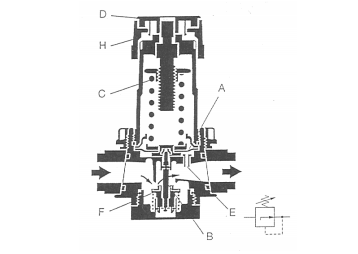
\includegraphics{regulator.png}
\end{figure}

\subsection{Cycle}

A pneumatic cycle is shown in Figure \ref{cycle}. It is asked to:
\begin{itemize}
    \item give the name of this cycle (square, L, U, \dots)
    \item give its sequence in one line
    \item differentiate the monostable and bistable components of the circuit.
\end{itemize}
Then:
\begin{itemize}
    \item give the motion diagram
    \item write all the functions ($f(\dots) = \dots$)
    \item \textit{simply and clearly} write this cycle in a GRAFCET program.
\end{itemize}

\begin{figure}[H]
    \centering
    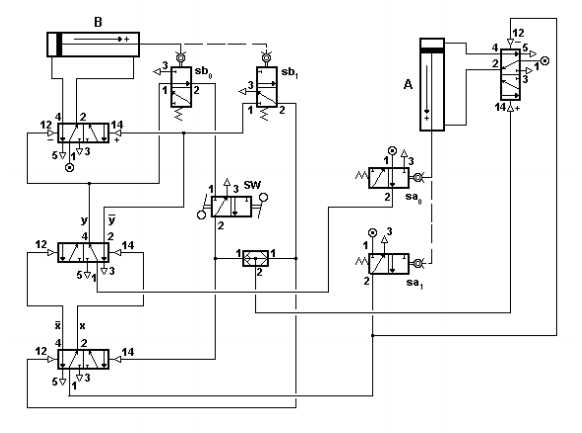
\includegraphics{Ucycle.png}
    \caption{Pneumatic cycle}
    \label{cycle}
\end{figure}

\subsection{Theory II}

What does represent these symbols? Insert your answer in the right column of the table (be concise).

\begin{figure}[H]
    \centering
    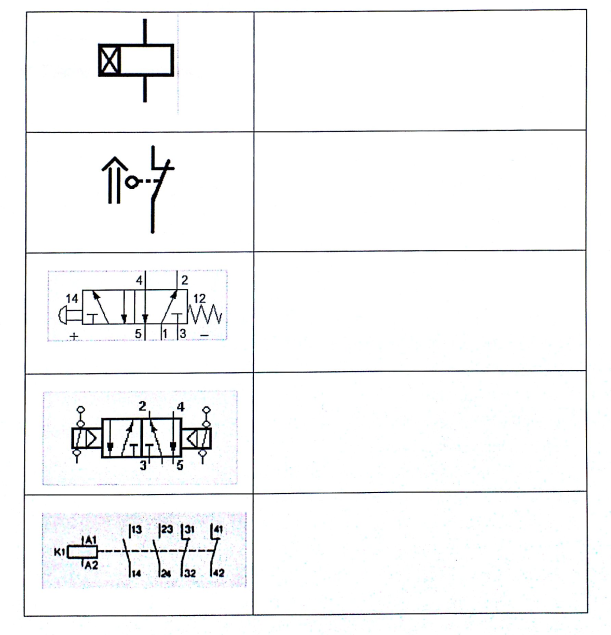
\includegraphics[width=0.7\textwidth]{symboles.png}
\end{figure}

\nosolution

\section{Sensors part}

We want to regulate the temperature in a tank that contains a product for hair. It is maintained at \SI{60}{\degree C} with a maximal variation of \SI{1}{\%}.

\begin{enumerate}
    \item Give two temperature sensors, explain briefly their principle and characteristics.
    \item Between these two sensors, choose the most appropriate one for this situation, and explain your choice.
\end{enumerate}

\nosolution

\end{document}
